\documentclass[11pt, a4paper]{article}
\usepackage[left=40mm, right=20mm, top=20mm, bottom=20mm, includefoot]{geometry}
\usepackage{setspace}
\usepackage{graphicx}
\usepackage{ulem} 
\usepackage[english]{babel}
\usepackage[autostyle]{csquotes}
\usepackage{listings}
\usepackage[style=apa,backend=biber, language=english]{biblatex}
\usepackage{url}
\addbibresource{sources.bib}
\setlength{\parindent}{0ex}
\setlength{\parskip}{1.5ex}
\font\titlefont=cmr10 at 18pt
\MakeOuterQuote{"}

\lstset{
  frame=tb, % draw a frame at the top and bottom of the code block
  tabsize=4, % tab space width
  showstringspaces=false, % don't mark spaces in strings
  numbers=left, % display line numbers on the left
  commentstyle=\color{green}, % comment color
  keywordstyle=\color{blue}, % keyword color
  stringstyle=\color{red} % string color
}

\linespread{1.5}
\begin{document}

\title{\titlefont The path to the right decision: An investigation into using heuristic pathfinding algorithms for decision making}
\author{Ashley Smith}
\date{\today}
\maketitle
\thispagestyle{empty}

\renewcommand\abstractname{\textbf{Abstract}}
\begin{abstract}
Lorem ipsum dolor sit amet, consectetur adipiscing elit. Cras justo velit, vestibulum sit amet turpis in, interdum rhoncus magna. Proin pulvinar posuere iaculis. Duis vulputate tristique arcu, id pretium ante blandit ut. Vestibulum ante ipsum primis in faucibus orci luctus et ultrices posuere cubilia Curae; Nam augue tellus, mattis quis consequat id, facilisis eu lectus. Vivamus euismod non quam sed condimentum. Orci varius natoque penatibus et magnis dis parturient montes, nascetur ridiculus mus. Orci varius natoque penatibus et magnis dis parturient montes, nascetur ridiculus mus. Phasellus vitae consequat nisi. Morbi vulputate tellus ut nibh vulputate, vitae blandit ex faucibus.
\end{abstract}

\cleardoublepage
\setcounter{page}{1}
\pagenumbering{roman}
\tableofcontents

\cleardoublepage
\pagenumbering{arabic}
\setcounter{page}{1}
\section{Introduction}

\subsubsection{Video games and artificial intelligence}

Games are good for the global economy. \citeauthor{Newzoo} reports that in October 2019 the global games market was worth \$148 billion with mobile games accounting for 46\% of that. In order to remain competetive, developers are pushed to make bigger, better and more complex games. The evolution of the technologies available has allowed for a greater number of elements to be simulated in the game world which could potentially increase a game's worth (\cite{blow2004game}). The entry barrier to creating these good looking and well executed games has been lifted with the establishment of engines like Unity (\cite{Unity}) and Unreal (\cite{Unreal}) to the point where even non-programmers can get involved using textual or visual scripting.

For many years, only the game's graphics were considered important (\cite{yap2002grid}; \cite{blow2004game}), however, good physics systems or competent AI (Artificial Intelligence) are now recognised as a way of improving the end-user's experience just as much well (\cite{blow2004game}). Game AI is different from the normal, academic AI as it simulates behaviour and aims to be believable and fun, whereas an academic AI aims to achieve a level of intelligence or autonomy to excel at a given task (\cite{nareyek2004ai}, p.60).

\subsubsection{The need for game AI}

AI has multiple uses within a games context but the majority of use cases employ AI to control the characters featured in a level of the game. \citeauthor{laird2001human} (\citeyear{laird2001human}, p.16) said that whether these characters are replacements for opposing players or characters that act as companions, villains and plot devices, "human-level AI can expand the types of experiences people have playing computer games". Using AI opens up the opportunity for increasing the difficulty of the game, and could be perceived as the kind of challenges that make games fun (\cite{buro2004call}, p.2). \citeauthor{laird2001human} (\citeyear{laird2001human}, p.16) also hypothesised that utilising such an AI is a good step towards the development of enjoyable and challenging gameplay, and potentially to "completely new genres" (\cite{laird2001human}, p.17). 

 "Customers value great AI" (\cite{nareyek2004ai}, p.60) and so it's important to choose a suitable approach that fulfills the expectations of the player thus the requirements of the game (\cite{millington2019ai}, p.19). Academic AI can be made using algorithms inspired by biology such as neural networks or genetic algorithms and trained through iteratation or with datasets. These approaches aren't used in game AI because of the high requirements to train the AI to interact with a specific game (\cite{nareyek2004ai}, p.64), moreover, it is easy to train the AI to play too strongly ruin the game (\cite{tozour2002evolution}, p.13). Instead, game AI developers embrace simpler, non-learning algorithms due to them being easier to understand, implement and debug (\cite{tozour2002evolution}, p.7).

 \subsubsection{Approaches to game AI development}

The most basic forms of AI used in games take the form of a series of if-then statements and are known as a 'production rule systems' (\cite{tozour2002evolution}). These statements are organised in a list and the AI uses the behaviour of the rules that evaluate to $true$. The result is a very basic AI that is not only limited to what actions it can take but also when it can take them. Similarly, decision trees combine the same if-then style with branching structures to create game AI (\cite{nareyek2004ai}, p.62), and the tree and subtrees are recursively traversed until a leaf node is found with the desired behaviour. This process is very easy to understand and implement (\cite{millington2019ai}, p.295), and the branching structure makes visualisation of the process more intuitive than the basic list used in a production rule system. Because of this, many consider decision trees to be one of, if not the simplest techiques to making AI (\cite{millington2019ai}, p.295; \cite{tozour2002evolution}, p.7).

FSMs, or Finite State Machines, are the most common approach to game AI (\cite{orkin2006three}, p.1; \cite{millington2019ai}, p309) due to being easy to understand and the efficacy of their output. FSMs consist of a directed graph where each node represents a state and the edges represent the transitions between them (\cite{tozour2002evolution}, p.6). A character can only be in one state at time and has no memory of any previous states (\cite{colledanchise2014performance}); each state represents an expected behaviour and determines what they do and the conditions to switch to a different state (\cite{diller2004behavior}, p.3). In the right environment, the impression of a well thought out FSM could compete with that a neural network, at a fraction of the time and resource costs, despite not always arriving at the optimal decisions (\cite{sweetser2002current}). However, each new behaviour requires the creation of a new state and the conditions of which this state integrates and transitions into other states, making expansion and maintainance cumbersome (\cite{sweetser2002current}, p.2; \cite{lim2010evolving}, p.3). There's no easy way to combine the tests inside of FSMs and selecting the conditions for a state transition is still very much a process that must be done by hand (\cite{millington2019ai}, p.313). 

The need for more flexibility in game AI has lead to the creation adaptation of modular algorithms such as behaviour trees (\cite{lim2010evolving}, p.1). Like decision trees, the recursive structure of a behaviour tree is simple to understand and implement while also being high level, allowing for more sophisticated AI to be created in a modular fashion through the use of subtrees and different node types (\cite{shoulson2011parameterizing}, p.144), each performs an action or check and then proceeds to succeed or fail (\cite{lim2010evolving}, p.4. It is these types that make the AI process at a higher level than standard decision trees, and when combined with leaf nodes that perform checks and actions to build trees, and then combined again to make trees containing subtrees, the simplicity and elegance of this technique certainly demonstrates why behaviour trees are getting attention (\cite{shoulson2011parameterizing}, p.144).

\subsubsection{The relationship of pathfinding and game AI}

One common requirement for game AI is for the characters to be able to traverse the areas of the game in a way which meets the player's expectations logically and efficiently - a task known as pathfinding. Regardless of what an AI decides to do, a pathfinding mechanic needs to be in place to allow the AI to navigate to where it needs to go, maneuvering around obstacles while still taking a sensible route (\cite{graham2003pathfinding}, p.60). For most games, the algorithm of choice is A* as it is the de-facto standard pathfinding algorithm (\cite{millington2019ai}, p.197; \cite{botea2004near}, p.2; \cite{nareyek2004ai}, p.64; \cite{leigh2007using}, p.73).

The A* algorithm analyses the game's map and generates a path from one location to another while minimising a $cost$ value - this value can represent anything but usually it represents the time or distance to travel along a given route (\cite{yap2002grid}, p.44). This means that the pathfinding algorithm itself doesn't decide where to go, only how to get there and the manner in which it does so. When asked to calculate a path, a pathfinding algorithm is provided a graph of nodes to determine which nodes can be reached from which (\cite{nareyek2004ai}, p.61). The algorithm isn't concerned with the what the data represents or in what form it is given, whether it is two-dimensional or three-dimensional, what the $cost$ is of travelling from one node to another, as long as it is equipped with the right functionality to digest this information (\cite{millington2019ai}, p.277; \cite{graham2003pathfinding}, p.60).

With the pathfinding process taking place after the decision has been made, the opportunity to involve the data gathered from pathfinding algorithm is missed. Often, the AI will decide to approach the nearest object, but obstacles in the way mean that the cost of navigating to the destination is greater than some alternative. While implementing the algorithm isn't difficult, ensuring the AI generates a path to the correct destination is difficult to do well (\cite{forbus2002qualitative}). Perhaps on the way to the destination, the character has to also navigate past traps or other hazards where it will need to decide whether to avoid or pass through - decisions that A* isn't fully equipped to deal with on it's own. If the AI wanted to factor in these hazards and real cost values, it would have to perform a more advanced check on where to travel too, maybe even using the pathfinding algorithm multiple times to definitely make sure that it wants to take the generated path, potentially ruining the game's performance.

Pathfinding algorithms are actually general purpose search algorithms applied to a spacial context (\cite{cui2011based}, p.125; \cite{orkin2003applying}, p.6; \cite{yap2002grid}, p.46); there is no such restriction that these algorithms should be restricted to pathfinding when in a games context. \citeauthor{millington2019ai} (\citeyear{millington2019ai}, p.197) said that "pathfinding can also be placed in the driving seat, making decisions about where to move as well as how to get there". With search algorithms having the flexibility of being able to traverse graphs of nodes representing any kind of data, it's no stretch to imagine the A* search algorithm being applied to a graph containing the same tests and actions found in decision and behaviour trees in order to generate a 'path' of actions rather than a path of spacial data (\cite{higgins2002generic}, p.114). This is paper aims to investigate and re-engineer A* to make decisions rather than paths in a game context.

\subsection{Literature Review (11-12 pages)}

\subsubsection{Dijkstra's algorithm: A graph and tree search algorithm}

A search algorithm is a recursive method designed to find a match for a piece of data within a collection such as an array, graph or tree (\cite{friedman1976algorithm}). A piece of data is provided and the search algorithm typically returns whether it is present and it's location. (\citeauthor{dijkstra1959note})'s algorithm (\citeyear{dijkstra1959note}) is a search algorithm that operates on trees and graphs (which are then interpreted as trees). The algorithm calculates the shortest difference from any node on the graph to any other node, and can be terminated early to avoid unnecessary computation if a destination is provided and found.

Dijkstra's algorithm works through the recursive summation and comparison of distance values starting from the a given start node (\cite{dijkstra1959note}, p.269). Each neighbouring node is added to the \emph{open} list, then, the current node's distance from the start is added to the length between the current node and its neighbour. If this tentative value is lower than the current distance value of the neigbour, it replaces it. When all the neighbours have been considered, the node with the lowest tentative value on the graph is selected and permanently 'visited' and are removed from the \emph{open} list. (\cite{dijkstra1959note}). This process is repeated until either there are no \emph{open} nodes left or the destination, if provided, has been visited, and thus a path and the distance from the start to the destination can be retrieved. The problem with Dijkstra's algorithm is that it always selects the node with the lowest tentative distance value, meaning that the algorithm has no notion of direction and is calculating the lowest distance to nodes that may not be relevant to getting to the destination (\cite{millington2019ai}, p.214).

\subsubsection{A* algorithm: A heuristic best-first search algorithm}

A* is an improvement of Dijkstra's algorithm in this regard (\cite{hart1968formal}, p.101) - while it doesn't stray far from how Dijkstra's algorithm works in the sense that it operates using a tentative distance value and it keeps track of the nodes that have and haven't been visited, it does extend the algorithm using what's known as a heuristic approach (\cite{cui2011based}, p.126). "Heuristics are criteria, methods or principles for deciding which among several alternative courses of action promises to be the most effective in order to achieve some goal" (\cite{pearl1984heuristics}, p.3). This means that in a pathfinding situation, a heuristic function could estimate the distance to the goal, by ignoring walls and measuring in a straight line, to direct the algorithm in the right direction and avoid evaluating routes that travel in the wrong direction to make the process more efficient (\cite{cui2011based}, p.127). Heuristics enable A* to perform a best-first search (\cite{yap2002grid}, p46), as the heuristic now has the power to select which node is the best to evaluate and prioritise over the others (\cite{russell2016artificial}, p.94). A good heuristic algorithm should explore nodes that have the most potential for leading to the goal node (\cite{korf1985depth}).

When identifying the next node to expand, A* will take this heuristic distance into account using the formula $f(n) = g(n) + h(n)$ (\cite{hart1968formal}, p.102; \cite{russell2016artificial}, p.95), where $g(n)$ is the real distance the algorithm has calculated from the start node to node $n$ and is the distance to be minimised while finding the \emph{goal}, $h(n)$ is the \emph{heuristic} distance from the current node $n$ and the destination, and $f(n)$ is the combination of these two metrics forming an estimate of the distance from the start node to the destination if travelling through node $n$, also known as the \emph{fitness} value (\cite{hart1968formal}; \cite{millington2019ai}; \cite{graham2003pathfinding}, p.64). 

This heuristic component of A* transforms it into a family of algorithms where applying a different heuristic selects a different algorithm (\cite{hart1968formal}, p.107), moreover, implementing A* and using a heuristic that returns a constant value for all nodes reverts A* back into Dijkstra's algorithm (\cite{lester2005pathfinding}, p.10; \cite{millington2019ai}, p.237). Conversely, implementing a well-designed heuristic method can be used to guarantee optimal solutions, and using a heuristic that is somewhere in-between can output results with varying degrees of accuracy in exchange for faster exection (\cite{millington2019ai}, p.219).  The implementation of a good heuristic can be difficult, as making the heuristic take more factors into account for accuracy has the drawback of making the algorithm less efficient overall with the heuristic being frequently used throughout the process.

On the other hand, \citeauthor{graham2003pathfinding} (\citeyear{graham2003pathfinding}, p.68) argue that one of the constraints of games the industry is the "over-reliance" on the A* pathfinding algorithm and describe the development of its many extensions as a way of avoiding the discovery of new techniques. The pathfinding process can require a lot of CPU resources, sometimes to the point of stalling the game, when applied to larger graphs (\cite{cui2011based}, p.127; \cite{stentz1996map}, p.110; \cite{graham2003pathfinding}, p.67). This indicates that the performance of A* can vary depending on various factors, and is why it is important to optimise A* by selecting an suitable storage mechanism for the graph and internal node storage as well as using a reasonable heuristic that balances efficiency and efficacy (\cite{millington2019ai}, p.228).

\subsubsection{Processing a character's perception of the game world ready for AI}

Every approach to designing game AI needs to find a way to digest information about the character and its environment that is relevant to the decision making process, and selecting this information is just as important as the form it is delivered in (\cite{cui2011based}, p.126). This digestion can vary in difficulty (\cite{diller2004behavior}, p.3) and is done for both performance and gameplay needs and all game AI solutions need the world to be re-interpreted to be better suited for both decision making (\cite{buro2004call}, p.2) and pathfinding (\cite{diller2004behavior}, p.3). Particular geometry of the map may need to be interpreted as vantage points, choke points or safe spots; particular formations of enemy units may need to be not only counted but also assessed for tactical strengths, whether engaging the units head-on is better than running away to a better location, and finally, the interpretation of time such as whether there is enough time to navigate to what would otherwise be a better location for fighting the enemy (\cite{buro2004call}). An AI would then take this abstraction of the world, combine it with the character's data and then consider what the character should be doing - if the character is in an 'attacking' state and the player is nearby then the decision would involve getting into a position and hitting or shooting at the player. 

If A* is to be used for game AI it also needs to operate on non-positional data. In standard pathfinding, each node is a position in the world and the edges between these nodes are the movements to get from one to another. Substituting each node to be an AI state and each edge to be an action that causes transitions from one state to another creates a graph can that A* could process. The implementation the states and actions depend on the expectations of the AI - traditional pathfinding could be implemented by having a 'move to' action that changes the position variable in the character's state. Regardless, a graph consisting of these nodes could be difficult to process and reduce the speed of A*.

A* can suffer from performance problems when used with many agents at once, or with a large or inefficient graph of nodes (\cite{graham2003pathfinding}). Many solutions have been discovered to prevent or reduce the impact on performance - one such solution is known as hierarchical pathfinding, where the game's map is simplified into chunks, (\cite{cui2011based}, p.126). By simplifying a group or grid of nodes into a single node that represents the whole group (like a quadtree), the pathfinding process can be applied to larger worlds as if they were actually smaller (\cite{botea2004near}). This works well for standard pathfinding, but if A* is applied to something other than purely spacial world data then the nodes need extra consideration. 

There is a large amount of actions a character can take at any given moment (\cite{nareyek2004ai}, p.62) and so applying a search algorithm to such a large set of tasks will make the process a lot slower than traditional methods if left unchecked. Hierarchical pathfinding essentially creates more nodes to expand in the short term to reduce the total number of nodes expanded in the long term and gain a net increase in performance, and so in order to apply it to a character's state instead of the world, nodes would have to be grouped by other metrics that aren't necessarily distance, such as 'attacking' actions and 'defending' actions. Splitting the world state gameplay elements like this can get complicated - what if a certain unit in a strategy game can attack from a longer range, would attacking the enemy from a distance be a defensive maneuver or an offensive one, and how easy is this to change on a per-unit basis (\cite{weber2011building})?

\subsubsection{Decision making with A* using GOAP}

\citeauthor{orkin2003applying} (\citeyear{orkin2003applying}, p.11) expressed that expectations of AI are growing with the release of every new game and that "we need to look toward more structured, formalized solutions to creating scalable, maintainable and re-usable decision making systems". Techniques used to create the Game AI featured in most games do not contain the scalability \citeauthor{orkin2003applying} envisions (\cite{laird2001human}, p.17), however, \citeauthor{higgins2002generic} (\citeyear{higgins2002generic}, p.117) declares that a pathfinding engine can be created generically, especially if a templated language is used, to give the code even more reusability. Implementing A* in this way would allow it to be used for both regular pathfinding and anything else that could requires searching (\cite{higgins2002generic}, p.120). With A* being efficient and optimisable (\cite{millington2019ai}, p.215), reusing A* for game AI has the potential to bring the benefits it usually brings to pathfinding to AI while being adaptable enough to scale up and meet expectations.

Orkin (\citeyear{orkin2006three}, p.1) worked on the development of the game AI for the game F.E.A.R (\cite{FEAR}). The approach used for this AI was called GOAP which stands for 'Goal Oriented Action Planning' and uses the A* algorithm as part of its decision making process and "allows characters to decide not only what to do, but how to do it" (\cite{orkin2003applying}, p.1). GOAP changes the data to be processed by A* from spacial data such as coordinates into character AI state data, such as what is found in FSMs. Therefore, the output of A* is no longer a sequence of movements but a sequence of actions also known as a plan (\cite{orkin2003applying}, p.2; \cite{tozour2002evolution}, p.6).

GOAP essentially takes the idea of having state machines to encapsulate behaviours and replaces the hand-programming the conditions and connections of state transitions with a pathfinding process with the aim being the decoupling of states and their transitions (\cite{orkin2003applying}, p.2). The pathfinding process uses each node to represent a state and the edges between each node as the actions that lead to those states (\cite{orkin2003applying}, p.7) When GOAP is used, a goal is given for the character to achieve which gives the AI some direction and what is returned is the sequence of actions that will satisfy the goal (\cite{orkin2003applying}, p.1). An action is a representation of one thing the character will do to change the world in some way, like opening a door or picking up a weapon (\cite{orkin2003applying}, p.2); some actions have preconditions that require the execution of another action prior to it (\cite{orkin2003applying}, p.5). A* will then find the sequence of actions, the plan, that satisfies the character's goal while minimising an arbitrary $cost$ value - \citeauthor{orkin2003applying} (\citeyear{orkin2003applying}, p.4 - p.5) suggests that this process creates interesting character AI that can adapt to change while also having a code structure that is reusable, maintainable and "elegant".

\begin{figure}[h]
  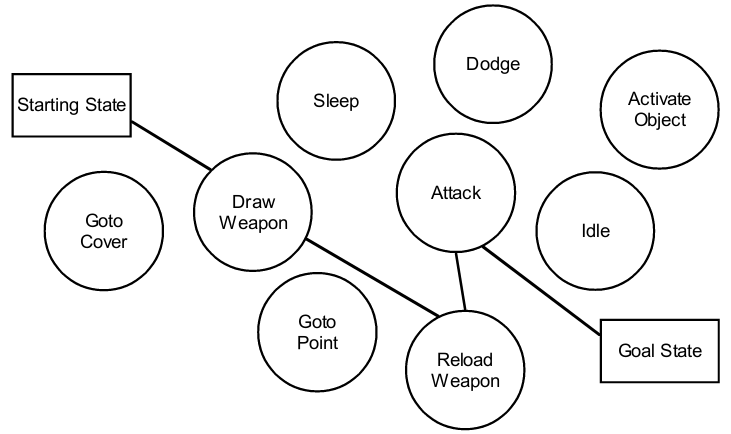
\includegraphics[width=\linewidth]{img/goap_figure_1.png}
  \caption{An example of GOAP (\cite{orkin2003applying}, p.3)}
  \label{fig:goap}
\end{figure}

A* being used in GOAP means that fundamental formula $f(n) = g(n) + h(n)$ (\cite{hart1968formal}, p.102) to be implemented: the calculation of a node's $fitness$ to determine the $cost$ of the actions taken up to that point and a heuristic function to determine the $cost$ of getting to the goal from a given node (\cite{orkin2003applying}, p.7). \citeauthor{orkin2003applying} (\citeyear{orkin2003applying}, p.7) also shares that the heuristic in GOAP can be calculated as the summation of unmet conditions of the goal node, but this is rather unclear. Given the example in figure \ref{fig:goap}, "the goal is to kill an enemy" (\cite{orkin2003applying}, p.3) could be interpreted in various ways that all seem unsuitable. If the goal condition is that the enemy is dead, the heuristic would be the same for all nodes but the goal state, making it potentially wasteful like Dijkstra's algorithm (\cite{millington2019ai}, p.214). Alternatively, if the condition was divided into multiple conditions such as the weapon needing to be drawn, the weapon needing to be loaded, and the enemy being dead, it is implied that either the algorithm has been run previously to determine the requirements of killing an enemy, or that they were programmed by the programmer - how would the starting state know that the weapon needed to be reloaded before drawing it? While GOAP does seem elegant, the graph in figure \ref{fig:goap} doesn't have a sizeable number of nodes; using dijkstra's algorithm wouldn't incur much of a performance cost with a graph this size. \citeauthor{orkin2003applying} (\citeyear{orkin2003applying}) suggests that a regressive search by starting at the goal and pathing to the start makes sense, and in figure \ref{fig:goap}, it does, as only one action can attack and so it's clear that the decision making process boils down to the character attacking the enemy.

Another problem of GOAP is that the high-level nature of the approach may not allow for enough control of the game (\cite{stanciu2012implementing}, p.87) - while making abstractions of the world is necessary for AI to process the information (\cite{buro2004call}, p.2) and thinking on a higher level is beneficial for making more humanlike decisions, the precision of the actions taken by the AI is both low level and very noticeable if incorrect (\cite{graham2003pathfinding}, p.60). Figure \ref{fig:goap} shows a decision making process that decides what to do but not necessarily where to do it. When the action "Goto Point" in figure \ref{fig:goap} gets executed, there's no indication of how the destinations are generated other than satisfying the preconditions for another action (for example, moving to an object to activate it) (\cite{orkin2003applying}, p.7). 

This isn't specific to GOAP as it applies to every AI approach where the generation of these locations isn't part of the AI. Is the character's AI deciding where to go, or just deciding that it has to go somewhere? In order for "Goto Cover" to act in a similar way to the "Goto Point" action, a goal or action precondition would either have to require the character to be out of line-of-sight, or be using one of the designated cover spots - this is how F.E.A.R (\citeyear{FEAR}) did it (\cite{orkin2006three}, p.12). The latter of these would require set locations to be marked as points of interest and then A* would be employed to find which coverspot would be the quickest to navigate to. The former would require calculating the closest position that allows the escape of line-of-sight. Both of these would have their own problems, and wrapping the entire pathfinding process as a single action would mean that the information from the pathfinding request would not be used in the decision making at all. Without utilising the AI's ability to create an impression of thought, the information given to these actions could be poorly chosen and "may be perceived as a lack of intelligence by a human player" (\cite{graham2003pathfinding}, p.63). To circumvent this, multiple "Goto Point" actions would be needed so that the planning system can evaluate each point into the workflow, but this could introduce its own problems without a well-designed heuristic that can distinguish between the different locations.

\subsubsection{Defining the notion of cost}

$Cost$, sometimes referred to as weight, is a term that will continue to be used when talking about A* as it is the the metric that governs the searching process (\cite{korf1985depth}). $Cost$ doesn't have to be a numeric value, as long as it can be compared and combined correctly with other $cost$ values, however, one numeric restriction of cost is that it cannot, or rather should not, be negative. The method A* uses to determine if a route should be expanded before another is if its $cost$ value is lower - when only positive values are added together it is assumed that there isn't a way for a $cost$ to decrease in value. While in mathematics it is entirely possible and valid for these values to be negative, the problems that make this necessary are not applicable to games (\cite{millington2019ai}, p.202).

In the formula $f(n) = g(n) + h(n)$ (\cite{hart1968formal}), each function returns a $cost$ - the combination of the goal and heuristic $cost$ values, also known as the fitness value, is used select the next open node to evaluate (\cite{russell2016artificial}, p.94). If $a$ and $b$ are two nodes in a graph and $f(a) < f(b)$, A* will interpret this as node $a$ being a more logical choice to expand (\cite{orkin2003applying}, p.7). Node $b$ won't be evaluated unless the route derived from node $a$ results in dead ends or more routes which have worse fitness values than node $b$. With the order of execution being so dependent on $f(n)$, it is important that the definition of the $cost$ of an action is calculated correctly. It is difficult to design such a system when everything is arbitrary, but metrics such as distance can be used to prioritise actions with lower distances such as movement; resources such as gold or mana could be used in game specific interactions to minimise spending important resource, and the time spent doing the action can also be factored in to drive the character to resolve the situation as quickly as possible (\cite{lester2005pathfinding}, p.8). \citeauthor{millington2019ai} (\citeyear{millington2019ai}) said that "the cost function is a blend of many different concerns, and there can be different cost functions for different characters in a game" and that this is called "tactical pathfinding". The ability to change the $cost$ per character further demonstrates the adaptability of A* - changing the way a character interacts with the world is just changing these $cost$ functions so that the A* prioritises one action over another.

Some decisions are more troublesome to weigh than others. With the constraint of no-negativity, what would the $cost$ be of an ability that regenerates mana instead of expends it? The only way apply reductions to values in this way would be to have a baseline $cost$ for an action and then add or subtract from it, however, this does mean that this baseline value would dictate the maximum value of the reduction and so forward planning is necessary to ensure that all reductions can be applied in a balanced way. Another difficult type of decision to way are ones that don't have inherent characteristics; with a good goal for AI being unpredictable, surprising behaviour (\cite{scott2002illusion}, p17), how would the incentive for performing strategies like flanking and ambushing be created, and how would it compare to the $cost$ for attacking an enemy directly head-on? \citeauthor{orkin2006three} (\citeyear{orkin2006three}, p.14) said that in F.E.A.R (\cite{FEAR}) this behaviour just came naturally from using a dynamic decision making system such as GOAP and that while they were prepared to implement "complex squad behaviour", none was implemented. The squad's ability to ambush "emerged" and gave illusion of complex behaviour.

\citeauthor{harmon2002economic} (\citeyear{harmon2002economic}, p.405) suggests that an "opportunity cost" could be introduced which represents the other actions that cannot be taken as a result of taking the given, mutually exclusive action, the objective being to apply penalties to actions due to the fact that an alternative and possibly better course of action is available. While this makes sense when it is difficult to reward the AI for performing these strategies, but adding penalties to other actions could get complex, there is no discussion of this concept from \citeauthor{orkin2006three} (\citeyear{orkin2006three}) from his work on F.E.A.R. Although, it is unclear whether \citeauthor{harmon2002economic} means to apply penalties based on the current action or the other actions, and if it's the latter, is this a flat $cost$ shared amongst all actions or does it try to give smaller penalties to the better tasks somehow? Regardless, to calculate this $cost$ some mechanism of the AI, such as the weighting function used to determine $g(n)$ or possibly the nodes themselves, needs to have knowledge of other nodes so that this opportunity cost can be determined and used, yet again requiring forward planning.

GOAP uses a simple "action cost" system to prioritise which tasks to carry out first (\cite{orkin2006three}, p.11). Using an integer or floating point value is ideal for the type of $cost$ as it can be added and compared with other values trivially. However, GOAP's method of creating unique characters is to assign different actions to make them act differently (\cite{orkin2006three}, p.8) as opposed to having them evaluate situations differently such as how \citeauthor{millington2019ai} (\citeyear{millington2019ai}) suggested. Giving characters different actions will implicitly change how they prioritise the same situation as they will be given new routes to explore, and for most games this might be the best idea. It could be a good idea to split the $cost$ type into a struct or array of values to give actions different values. Throwing a grenade and shooting a pistol could be considered equivalent in difficulty to perform, but typically grenades have more firepower in exchange for there being less available; reducing these actions to a single value could be difficult depending on how you look at it, but splitting the value into a struct would allow the programmers to keep track of firepower and usage penalties seperately. When needed for comparison, this struct would evaluate to the sum of it's parts - but certain characters or situations could choose to adjust or completely omit parts of the $cost$ so that actions are percieved in different ways depending on how a character views a certain cost. For a fast character, the $cost$ to move might be halved and the $cost$ of being exposed doubled in order to give the impression of an agile and hard-to-hit character.

\subsubsection{Selecting a goal}

When the game world has been processed, the actions a character can perform have been laid out and the methods of evaluating courses of action have been provided, the only things remaining that A* needs to function are the start and goal node states for the actual decision. The starting state is trivial as it is simply the current state of the character and world; the goal state node requires more consideration than that though. In standard pathfinding, the output is the shortest path from the starting node to the goal node, if such a path exists (\cite{nareyek2004ai}, p.61). For game AI though, the goal needs to represent how the character or world should be - or rather the objective outcome of the decision making process. This objective can be difficult to ascertain as a goal node could represent anything; what seems to be a simple goal such 'win the game' becomes a rigorous series of tests to both calculate the $cost$ reaching the goal than another (\cite{harmon2002economic}, p.403). On the other hand, objectives that are too small or disconnected may not combine correctly to form this over-arching goal of winning the game. A balance is needed, whether that means the objective is to chase the player or defend an area, the objective needs to be focused on winning without being vague.

While \citeauthor{orkin2003applying} (\citeyear{orkin2003applying}) talks about in great depth about how GOAP handles making a decision to satisfy goal conditions, but doesn't describe where these objectives come from. A "squad coordinator" is mentioned (\cite{orkin2003applying}, p.13) that organises multiple agents into squads when they're close together, but the actual goals of the AI can come from both the character's individual AI and the squad coordinator. GOAP doesn't replace an FSM, so it could be inferred that the character's state when a goal is reached determines the next goal and thus the character's behaviour, with the initial state being defaulted, scripted or randomised (\cite{orkin2003applying}, p.2). Alternatively, game AI could be created in layers, and the output of one layer could be the desired goal of another, but this would mean that this problem propagates to the highest level. 

Another talking point regarding goals is the amount of designated goal state nodes in the graph. There is typically only a single goal in standard pathfinding, but it is possible, maybe even advantageous, for some games to contain multiple goal nodes in a graph (\cite{millington2019ai}, p.272). Instead of checking for a match with a certain location (or state, when developing AI), a method that checks whether a given node meets the requirements of being classified as a goal could be used instead; the heuristic would also need revision as it would need to calculate the heuristic $cost$ to reach the 'nearest' goal rather than just the single, given goal (\cite{millington2019ai}, p.272). Having multiple goals would grant the ability for the AI to re-route to a different goal if it's easier, but this comes at a cost of a more intricate and potentially confusing implementation and design of the AI as well creating a balancing issue to make sure goals are chosen as expected by players.

\subsubsection{Summary}

END

In this paper, the mechanisms of the A* search algorithm are examined and re-engineered, through the substitution of input and output types, to investigate the modularity and adaptability of an AI made in this way. The aim of using this approach is to bring decision-making and pathfinding closer together and therefore simplifying the overarching process of perceiving, deciding and interacting in the game world.

\subsection{Methods and Methodologies}

\section {Design, Development and Evaluation}

\section{Design (14-15 pages when combined with development)}

\subsection {Development (14-15 pages when combined with design)}

\subsection {Results and Evaluation (11-12 pages including critical review)}

\section {Conclusions}

\subsection {Conclusions and Critical Review}

\printbibliography
\end{document}
